\chapter{Evaluation of results}
The goal of this chapter is to perform a rigorous evaluation of the created aspect-based sentiment analysis algorithm. First, the numerical scores of each criterion estimated by the algorithm are compared to the scores given to these criteria by the reviewers. Then, the algorithm's output is evaluated in more detail, by establishing the precision and recall of aspect identification and the accuracy of the sentiment analysis, using an annotated set of reviews. Finally, the results of the evaluation are discussed and suggestions are made for future improvements.
\section{Evaluation using reviews with numerical scores}
The reviews from ISWC 2018 contain numerical scores for a wide range of criteria as was mentioned in section \ref{sec:rev_structure}. It was decided to compare the numerical scores outputted by the sentiment analysis algorithm with the ground-truth scores taken from the reviews. Because the ISWC set of criteria is more detailed that the set of criteria the algorithm works with, it was necessary to create a mapping between them which you can see in Table \ref{tab:mapping_numerical}. 

\begin{table}[!htb]
\caption{Mapping between the chosen set of criteria and ISWC 2018 criteria}
\centering
\label{tab:mapping_numerical}
\begin{tabular}{l|l}
\textbf{Algorithm's criteria} & \textbf{ISWC 2018 criteria}    \\ \hline
relevance                     & appropriateness                \\
novelty                       & originality/innovativeness     \\
                              & impact of ideas and results    \\
technical quality             & implementation and soundness   \\
state of the art              & related work                   \\
evaluation                    & evaluation                     \\
presentation                  & clarity and quality of writing
\end{tabular}
\end{table}

The numerical output was evaluated using the mean absolute error function (MAE), which measures the absolute average distance between the real data $Y$ and the predicted data $\bar{Y}$:

\begin{equation}
MAE = \frac{1}{n} \times \sum_{i=1}^{n} \lvert Y_{i} - \bar{Y_{i}} \rvert
\end{equation}


The MAE was calculated separately for each criterion to see if the algorithm performs better or worse for some of them. The default range of [1;5] for scores outputted by the algorithm was matched to the [-2;2] range of the ISWC reviews. Because the algorithm outputs ``n/a'' instead of a number for criteria for which no sentiment value was found,  the number of times the ``n/a'' value occurs for each criterion was also calculated.

The results of the numerical evaluation carried over the 20 ISWC 2018 reviews can be seen in Table \ref{tab:eval_numerical}. It is clear that the algorithm often struggles with finding any criterion score, especially when it comes to relevance, novelty and technical quality. Even when it does give a numerical score, it is often fairly off. This could have several explanations. Firstly it is possible that when reviewers have the option of expressing their opinion numerically, they sometimes do not feel the need to also give a more elaborate explanation. The second explanation is that the algorithm simply does not perform well when it comes to discovering aspect expressions and/or sentiment words. This is studied more closely in the next section, where the results are evaluated on the sentence level. 

Another issue might be the way in which the numerical scores are estimated -- each time an aspect expression is discovered and assigned a polarity of +1 or -1 the value is added to the respective criterion score. Finally the scores are averaged by the number of times a value was added and normalized to a given score range. Therefore, if for a criterion only one aspect expression is found with a given polarity the final score will always be an extreme in the score range, but that is a much rarer occurrence in the scores given by human reviewers. To check if this might be the issue it was tested by changing the normalization of polarity to four different values, where a criterion is added a score of +1 if the orientation of an aspect expression is higher than 0.5, a score of +0.5 if the orientation is higher that 0 and analogously the -0.5 and -1 scores for negative orientations. The results after that change can be seen in Table \ref{tab:eval_numerical_granular}. It is apparent that this leads to better results and so a more fine-grained approach to polarity is necessary.



\begin{table}[!htb]
\caption{Results of the numerical evaluation of ISWC 2018 reviews}
\label{tab:eval_numerical}
\centering
\begin{tabular}{l|D{.}{.}{2}|c}
\textbf{Criterion} & \textbf{MAE} & \textbf{Number of missing values} \\ \hline
relevance          & 1.44         & 11                                \\
novelty            & 1.68          & 0                                \\
technical quality  & 1.64         & 9                                \\
state of the art   & 1.38          & 4                                 \\
evaluation         & 1.35          & 3                                 \\
presentation       & 0.94          & 4 
\end{tabular}
\end{table}

\begin{table}[!htb]
\caption{Results of the numerical evaluation of ISWC 2018 reviews using a more granular approach to polarity}
\label{tab:eval_numerical_granular}
\centering
\begin{tabular}{l|D{.}{.}{2}|c}
\textbf{Criterion} & \textbf{MAE} & \textbf{Number of missing values} \\ \hline
relevance          & 1.33        & 11                                \\
novelty            & 0.93          & 0
\\
technical quality  & 1.09         & 9                                \\
state of the art   & 1.06         & 4                                 \\
evaluation         & 0.82          & 3                                 \\
presentation       & 0.69          & 4                                
\end{tabular}
\end{table}

\section{Evaluation using annotated review comments}
As was stated in section \ref{sec:preprocessing_eval}, a dataset of reviews with comments annotated by criterion and sentiment was prepared in order to evaluate the accuracy of the algorithm in more detail. The goal was to determine the precision and recall of the algorithm as well as to take a closer look at where the algorithm struggles with accurate results. This section presents the outcome of the evaluation first for the criterion identification and then for the sentiment analysis.
\subsection{Evaluation of the criterion identification}
The annotated dataset was compared to the output of the sentiment analysis algorithm. 
Each annotated comment for which the appropriate criterion was found by the algorithm was classified as \textit{true positive} (TP), each comment which was labeled by a criterion but the algorithm did not discover it was labeled by \textit{false negative} (FN) and each time the algorithm outputted a criterion incorrectly (it was not labeled with the same criterion by the annotators) it was classified as \textit{false positive} (FP). Because sometimes a comment was labeled differently by each annotator and they did not reach an agreement during the annotation phase, a comment was labeled as TP if the algorithm outputted either one of the annotated criteria. Also it is important to note that while the annotators labeled comments which sometimes consist of multiple sentences, the algorithm works on a sentence level. Therefore, the outputted sentences and their criteria were grouped for the evaluation to match the comments.

Some of the reviews contain numerical scores for the extracted criteria, however while the algorithm always correctly identifies the respective criteria, it is unable to assign a sentiment polarity based on the score value. Because each conference might use a different scale for these scores and the algorithm should work independently of any knowledge about the specific source of reviews, it was decided against using the scores for the sentiment analysis and instead only focus on the textual data. Therefore the parts of reviews with numerical scores were ignored for both the annotation and evaluation phase.

 The results of the comparison between annotated criteria and outputted criteria can be seen in Table \ref{tab:eval_ae}.
\begin{table}[htb!]
\caption{Evaluation of the criterion identification}
\label{tab:eval_ae}
\centering

\begin{tabular}{l|rrr}
\textbf{conference} & \textbf{TP} & \textbf{FP} & \textbf{FN} \\ \hline
ESWC 2019           & 17          & 15          & 14          \\
EKAW 2018           & 31          & 17          & 34          \\
ISWC 2018           & 22          & 20          & 13          \\ \hline
Total               & 70          & 52          & 61         
\end{tabular}
\end{table}

To quantify the accuracy of the results, first the precision for criteria over the entire dataset was calculated using the following equation:

\begin{equation}
precision = \frac{TP}{TP + FP}
\end{equation}

which resulted in a precision of $57.38$~\%. 

The recall for criteria over the entire dataset was calculated as:

\begin{equation}
recall = \frac{TP}{TP + FN}
\end{equation}

which evaluates the recall at $53.44$~\%.


Figure \ref{img:eval_ae} shows the contribution of each criterion to each of the evaluation label (TP, FP or FN), while Figure \ref{img:eval_ae_r} shows these results for each criterion individually by displaying the relative amount of each of the evaluation labels to their sum. The algorithm visibly struggles the most with discovering the \textit{technical quality} criterion, where the false negatives amount for 61~\% of the assigned evaluation labels, 25~\% were false positive and the algorithm succeeded in correctly finding the correct criterion in just 14~\% of cases. The algorithm also did not fare particularly well for the \textit{state of the art} criterion, where although the relative amount of false negatives is fairly small, the number of false positives is at 62~\%, meaning that a considerable amount of sentences get labeled with this criterion wrongly. 

 In terms of discovering the correct criteria, the \textit{presentation} criterion amounts for 37~\% of all true positives and the \textit{evaluation} criterion for 31~\%, however in 38~\% of all cases that \textit{evaluation} was assigned any of the evaluation labels, 31~\% were false positives, which is a fairly high amount even though the relative amount of true positives is 52~\%. 

Generally a considerable amount of false positives come from the fact that when a reviewer talks about some issue that falls under the \textit{presentation} criterion, they refer to some section of the paper by the section name or topic, which often falls under an aspect expression belonging to some other criterion. Consider the sentence \textit{``The section numbers appear off, too--the introduction says that evaluations are performed in Section 6, for instance, but it's actually in Section 5.''}, which for a human reader obviously mentions a problem with the quality of writing, however the algorithm picks up on the \textit{evaluations} keyword and incorrectly labels the sentence with the \textit{evaluation} criterion.  

Another issue that leads to a significant number of false positives is that at the beginning of most reviews, there is a summary of the paper, stating its objectives. These summaries often contain different aspect expressions, as there is an overlap between the criteria names or expressions and the general vocabulary of the field. 
For example, the sentence \textit{``To achieve this, an inference rule is translated into a SPARQL CONSTRUCT query that is evaluated against the schema of the RDF dataset.''} only mentions how the solution proposed in the reviewed paper works, it is not the reviewers comment on the quality of the actual evaluation but it gets recognized by the algorithm as such. Similarly the sentence \textit{``In this paper authors investigate how state-of-the art language technologies LT (tools, algorithms and resources) can be ported to the historical ecology domain.''} gets labeled with the \textit{state of the art} criterion, even though the sentence does not refer to how the reviewer feels about the research of the domain done by the authors (which would indeed fall under \textit{state of the art}). 

The false negatives, meaning cases where the annotators assigned a criterion to a comment but the algorithm did not, mostly come from the fact that the comments did not include any expressions that would immediately lead to a certain criterion. For instance in the case of the \textit{technical quality} aspect it would require a significantly more complex domain specific lexicon of technical terms to lessen the amount of false negative in sentences such as \textit{``Even if a rule is determined as potentially applicable after running the query derived from the rule on the data schema, the rule  cannot be executed until relevant instances are entered into the dataset.''}.

To explain the high amount of missing numerical values discovered in the previous section, the output of ISWC 2018 data was inspected and compared with the annotated dataset. It was discovered that out of the  7 ``n/a'' criteria values outputted for the 5 annotated reviews 4 criteria were also missing in the annotations (in other words according to the annotators there was no comment related to these criteria). All unknown values from the examined dataset belonged either under the \textit{relevance} criterion (4 unknown values and 3 reviews with no \textit{relevance} annotation) or the \textit{technical quality} criterion (3 unknown values and 1 review with no \textit{technical quality} annotation). As was already explained, the algorithm does not perform well in classifying comments regarding \textit{technical quality} which is likely the cause of the missing values. On the other hand \textit{relevance} has a significantly lower amount of false negatives, so it is more likely that reviewers simply do not feel the need to expand on their numerical score when this criterion is concerned.

\begin{figure}[H]
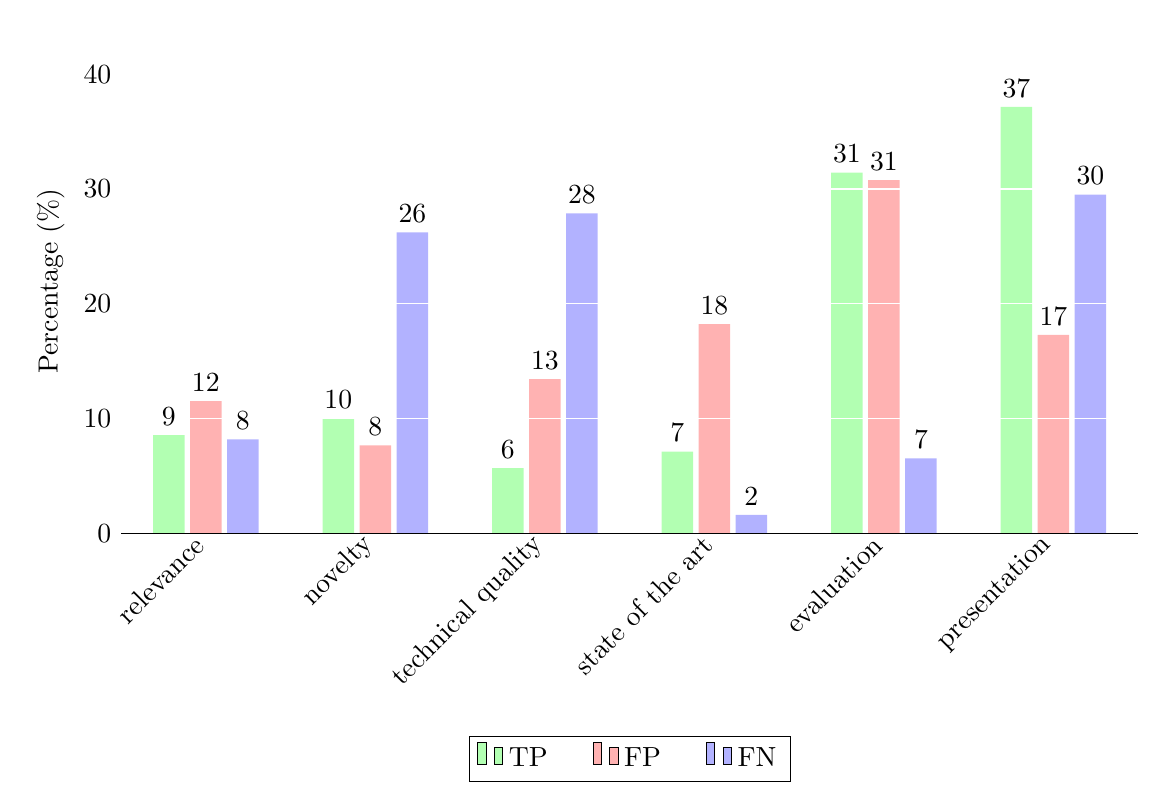
\begin{tikzpicture}
\begin{axis}[
        ybar, axis on top,
        height=8cm, width=14.5cm,
        bar width=0.4cm,
        ymajorgrids, tick align=inside,
        major grid style={draw=white},
        enlarge y limits={value=.1,upper},
        ymin=0, ymax=40,
        axis x line*=bottom,
        axis y line*=left,
        y axis line style={opacity=0},
        tickwidth=0pt,
        enlarge x limits=true,
        legend style={
            at={(0.5,-0.4)},
            anchor=north,
            legend columns=-1,
          /tikz/every even column/.append style={column sep=0.5cm}  
        },
        ylabel={Percentage (\%)},
        symbolic x coords={
         relevance,	novelty,	technical quality,	state of the art,	evaluation,	presentation
},
       xtick=data,
       x tick label style={rotate=45,anchor=east},
       nodes near coords={
        \pgfmathprintnumber[precision=0]{\pgfplotspointmeta}
       }
]
\addplot [draw=none, fill=green!30]
	coordinates {(relevance,8.57) (novelty,10)
		 (technical quality,5.71) (state of the art,7.14) (evaluation,31.43) (presentation,37.15)};
		 
\addplot [draw=none,fill=red!30] 
	coordinates {(relevance,11.54) (novelty,7.69)
		 (technical quality,13.46) (state of the art,18.23) (evaluation,30.77) (presentation,17.31)};
		 
\addplot [draw=none, fill=blue!30] 
	coordinates {(relevance,8.2) (novelty,26.23)
		 (technical quality,27.87) (state of the art,1.63) (evaluation,6.56) (presentation,29.51)};
\legend{TP,FP,FN}
\end{axis}
\end{tikzpicture}
\caption{Evaluation results based on the contribution of each criterion to the evaluation labels}
\label{img:eval_ae}
\end{figure}

\begin{figure}[H]
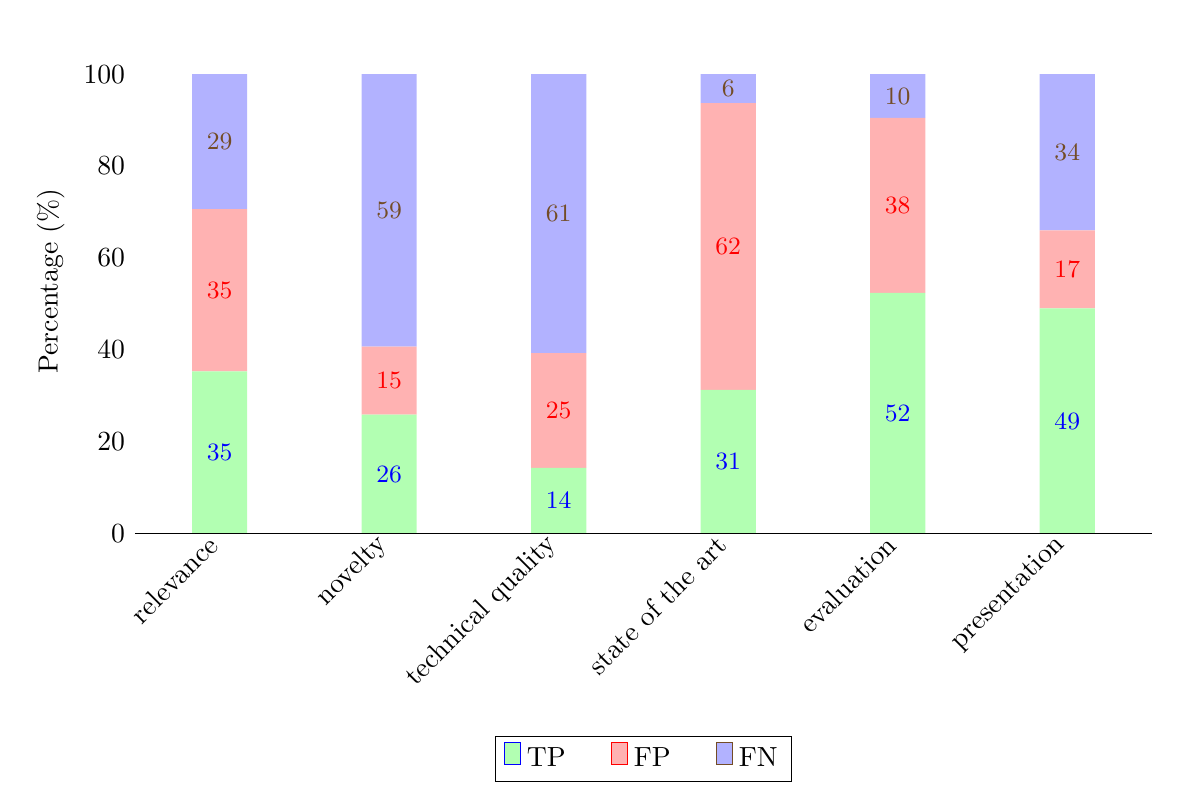
\begin{tikzpicture}
\begin{axis}[
        ybar stacked, axis on top,
        height=8cm, width=14.5cm,
        bar width=0.7cm,
        enlarge y limits={value=.1,upper},
        ymin=0, ymax=100,
        axis x line*=bottom,
        axis y line*=left,
        y axis line style={opacity=0},
        tickwidth=0pt,
        enlarge x limits=true,
        legend style={
            at={(0.5,-0.4)},
            anchor=north,
            legend columns=-1,
              /tikz/every even column/.append style={column sep=0.5cm} 
        },
        ylabel={Percentage (\%)},
        symbolic x coords={
         relevance,	novelty,	technical quality,	state of the art,	evaluation,	presentation
},
       xtick=data,
       x tick label style={rotate=45,anchor=east},
       nodes near coords={
        \pgfmathprintnumber[precision=0]{\pgfplotspointmeta}
       },
       nodes near coords style={font=\small}
]
\addplot+ [draw=none, fill=green!30, ybar]
	plot coordinates {(relevance,35.3) (novelty,25.9)
		 (technical quality,14.3) (state of the art,31.3) (evaluation,52.4) (presentation,49)};
		 
\addplot+ [draw=none,fill=red!30, ybar] 
	plot coordinates {(relevance,35.3) (novelty,14.8)
		 (technical quality,25) (state of the art,62.4) (evaluation,38.1) (presentation,17)};
		 
\addplot+ [draw=none, fill=blue!30, ybar]
	plot coordinates {(relevance,29.4) (novelty,59.3)
		 (technical quality,60.7) (state of the art,6.3) (evaluation,9.5) (presentation,34)};
\legend{TP,FP,FN}
\end{axis}
\end{tikzpicture}
\caption{Evaluation relative to the number of assigned evaluation labels of each criterion}
\label{img:eval_ae_r}
\end{figure}

\subsection{Sentiment analysis evaluation}
The comments with aspects that were correctly classified (those with the TP label) were also evaluated based on whether they were labeled with the correct sentiment. In the annotated dataset there was only one comment where the annotators did not reach an agreement on the appropriate sentiment -- \textit{``Though, this approach solves a relevant problem there are several concerns:''}. This was due to that comment  containing dual polarity which is an issue already pointed out in section \ref{sec:data_sl}. This comment could therefore be taken as either positive or negative  and was evaluated accordingly.

Over 75.7~\% of comments with correctly identified criterion were also correctly classified by sentiment while 24.3~\% were not. 

 Relative to the number of TP comments regarding a certain criterion the algorithm performs best for the sentiment analysis of the \textit{state of the art} criterion with an accuracy of 100~\% (see Figure \ref{img:eval_sa}), however since only 5 comments belonging to this criterion were correctly identified, the number might not be objectively accurate. Interestingly  the algorithm does well at determining the polarity of the \textit{presentation} criterion  as the comments tend to contain similar sentiment expression such as \textit{well-written} or \textit{clear} so due to their frequency across reviews they were picked up during the creation of the sentiment lexicon.

\begin{figure}[H]
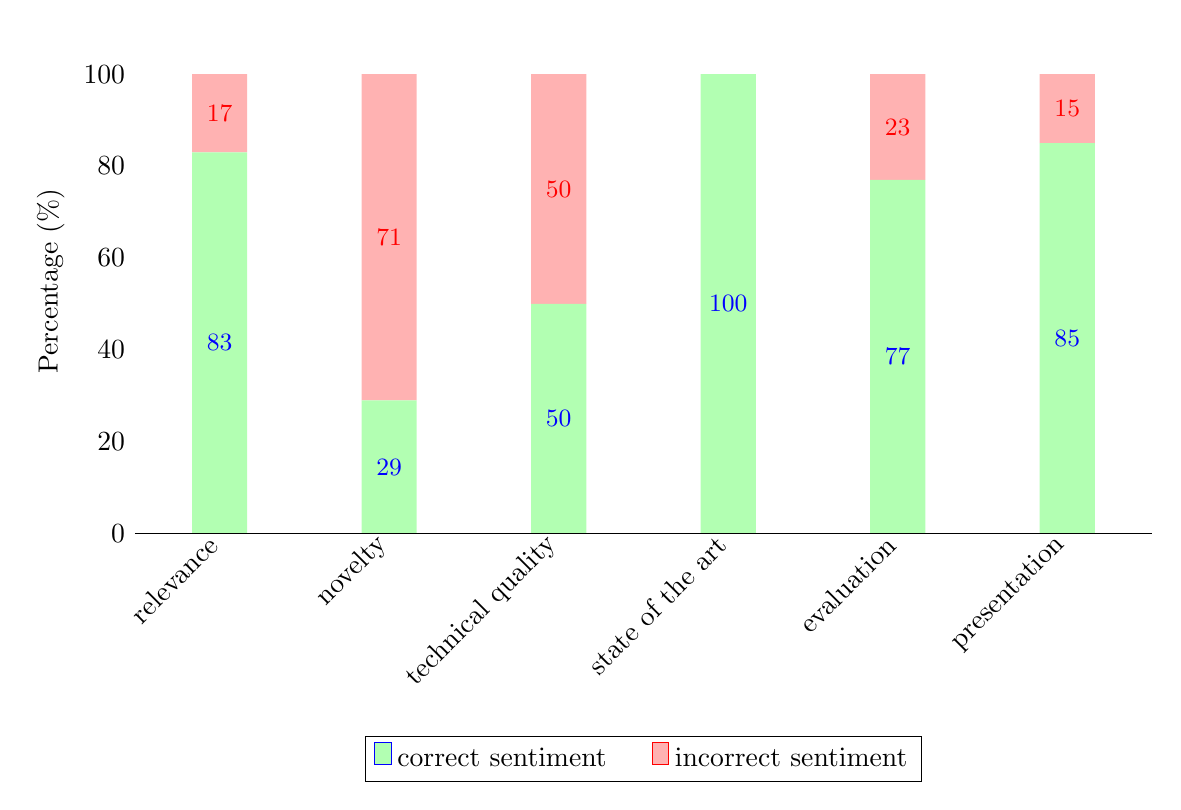
\begin{tikzpicture}
\begin{axis}[
        ybar stacked, axis on top,
        height=8cm, width=14.5cm,
        bar width=0.7cm,
        enlarge y limits={value=.1,upper},
        ymin=0, ymax=100,
        axis x line*=bottom,
        axis y line*=left,
        y axis line style={opacity=0},
        tickwidth=0pt,
        enlarge x limits=true,
        legend style={
            at={(0.5,-0.4)},
            anchor=north,
            legend columns=-1,
              /tikz/every even column/.append style={column sep=0.5cm} 
        },
        ylabel={Percentage (\%)},
        symbolic x coords={
         relevance,	novelty,	technical quality,	state of the art,	evaluation,	presentation
},
       xtick=data,
       x tick label style={rotate=45,anchor=east},
       nodes near coords={
        \pgfmathprintnumber[precision=0]{\pgfplotspointmeta}
       },
       nodes near coords style={font=\small}
]
\addplot+ [draw=none, fill=green!30, ybar]
	plot coordinates {(relevance,83) (novelty,29)
		 (technical quality,50) (state of the art,100) (evaluation,77) (presentation,85)};
		 
\addplot+ [draw=none,fill=red!30, ybar] 
	plot coordinates {(relevance,17) (novelty,71)
		 (technical quality,50) (state of the art,0) (evaluation,23) (presentation,15)};

\legend{correct sentiment, incorrect sentiment}
\end{axis}
\end{tikzpicture}
\caption{Results of sentiment analysis by criterion}
\label{img:eval_sa}
\end{figure}

\section{Discussion of results}

The comparison between the numerical output of the system with the numerical scores given in the reviews resulted in a mean average error of 0.99 on a scale from -2 to 2, meaning the algorithm was usually nearly one point off. This was deemed a significant error margin and in order to get more insight into the accuracy of the criterion identification and the sentiment analysis a more detailed assessment ensued on a sentence level which estimated the precision of the criterion identification at 57.38~\% and the recall at 53.44~\%. As such, the error rate is quite high, however even the annotators had a substantial level of disagreement, initially diverging in their criterion labeling in over a third of the comments. This suggests that reconstructing the intended meaning of the review comments is a particularly difficult task even for human annotators.

The accuracy of the sentiment analysis was calculated using a set of comments with correctly identified criterion determined by human reviewers. The system detected the accurate sentiment in more than 75~\% of executed cases. Notably, this is an improvement on the result of a similar sentiment analysis carried out in a comparable study with focus on peer reviews of scientific publications. This analysis algorithm only managed to reach an accuracy level of nearly 73~\% even though the sentiment analysis performed in this study was not aspect based \cite{nano_peer}, which makes determining the sentiment easier. Consider the sentence \textit{``While it is a fairly relevant topic, there were too many typos and the results were not at all evaluated against any of the existing state-of-the-art systems, so I do not consider the work mature enough for acceptance.''}.  The overall sentiment of the sentence is negative, as it presents more reasons for rejecting the paper rather than accepting it and for that same reason it would not be difficult for most dictionary-based sentiment analysis methods to correctly classify the sentence as negative. However, if we classify the sentiment on an aspect level, it is necessary to also find out which sentiment expressions of the sentence belong to which aspect, which in this case means it needs to recognize that even though the sentence contains more negative expressions, relevance is judged positively. 


The algorithm is capable of being substantially improved quite easily when given the availability of a significantly larger dataset. This could help put together both a better aspect expression dictionary and a vast sentiment lexicon. The creation of which heavily relies on the frequency of terms across reviews. Additionally, should a larger dataset be available, it would be possible to perform a more detailed exploration of the specificities of language used in similar data, creating a more complex algorithm using the discovered knowledge. 

Another possible way to improve the results would be to put together specialized rules for the different criteria. For example, as comments about the \textit{presentation} criterion often lead to false positives matches on other criteria, it would be possible to  create a rule where criteria expression found in a sentence where there is also a match on \textit{presentation} would be discarded. Another example of a criterion-specific rule would be to study the structure of a sentence in a more complex manner by using syntactic analysis, to for instance discover that in a sentence such as \textit{``The rule  cannot be executed until relevant instances are entered into the dataset.''} the adjective \textit{relevant} is connected to \textit{instances}, which is not a term related to the work itself and therefore the sentence should not be considered as a comment on the \textit{relevance} criterion. However, these rules would require to limit the algorithm to a specific set of criteria, which goes against the original idea to create an algorithm that could be reused on a number of different domains.

The sentiment analysis as well as criterion identification could also be enhanced by creating a sentiment lexicon specific to each criterion. Firstly, there are many sentiment expressions that are context-dependent: For example, \textit{small} would most likely considered a positive word in relation to an evaluation error but a negative one when commenting on the contribution of the work. This problem could be solved by having a dedicated sentiment lexicon for each criterion, and thus providing the necessary context. Secondly, some sentiment expressions have a strong connection to certain criteria. For example, \textit{clear} is almost exclusively used in relation with the \textit{presentation} criterion. This could be leveraged to aid in aspect identification, as a sentiment expression which is strongly related to a particular criterion could be used as an indication of its presence, if no criterion expression is found. 



